\chapter{Controlling Physical Systems}
\label{chap:pid}

\section{Introduction}

Computer programmers are accustomed to instructions that operate
\emph{instantaneously} and \emph{reliably}. Both assumptions fail when
writing code that controls a physical system. In this chapter we will
take the first steps towards writing programs that can reliably
control physical systems in an unpredictable world.

%% INTRODUCE PID CONTROLLER

\section{Open Loop Control}

\begin{figure}
\begin{center}
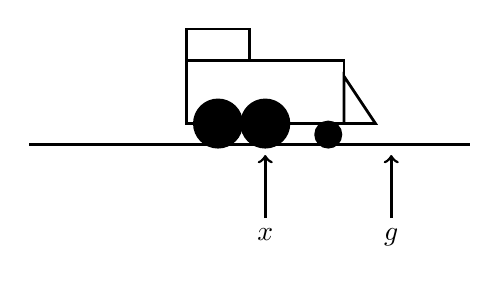
\begin{tikzpicture}
[line width=1pt,rotate=0,scale=.4]

\filldraw (2.0, 1) circle (.75);
\filldraw (3.5, 1.0) circle (.75);
\filldraw (5.5, .65) circle (.4);

\draw (1,1) -- (6,1) -- (6,3) -- (1, 3) -- cycle; %body
\draw (1,3) -- (3,3) -- (3,4) -- (1, 4) -- cycle; %cab
\draw (6,1) -- (7,1) -- (6,2.5)  -- cycle; %plow
\draw (-4, .325) -- (10, .325); %rails

\draw[->] (3.5, -2)  node [anchor=north]{$x$} -- (3.5,0);
\draw[->] (7.5, -2)  node [anchor=north]{$g$} -- (7.5,0);

\end{tikzpicture}
\end{center}
\caption{A self-driving locomotive.}
\label{fig:locomotive1}
\end{figure}


Consider the problem of programming a controller for the self-driving
locomotive in Figure \ref{fig:locomotive1}.  In this figure $x$
indicates the starting position of the locomotive and $g$ indicates
the goal location.

Our first attempt at developing a controller might look something like
the following:

\begin{minipage}[c]{0.95\textwidth}
\begin{lstlisting}[label={lst:open-loop},caption={Open Loop Control Algorithm}]
def open_loop(x, g):

    # Calculate the distance to travel.
    d = g - x

    # Cover that distance in one second.
    for one second:
        drive forward at a speed of d/second
\end{lstlisting}
\end{minipage}

Algorithm \ref{lst:open-loop} is an example of an \vocab{open loop
  controller}\index{open loop control}. Open-loop control involves
sending a sequence of control signals that, based on our understanding
of the system we are controlling, should move the system into the
target configuration.

There are problems with Algorithm \ref{lst:open-loop}.  First,
locomotives are \emph{heavy}.  The success of this algorithm relies on
the unrealistic assumption that we can instantaneously changing the
speed from zero to the desired value of $d/s$.  Second, even after the
locomotive reaches the target speed, factors like friction and
mechanical imperfections will make it impossible to perfectly maintain
that speed. Over time, small errors in speed will result in
significant errors in the final position.


\section{Closed Loop Control}

\begin{figure}
\begin{center}
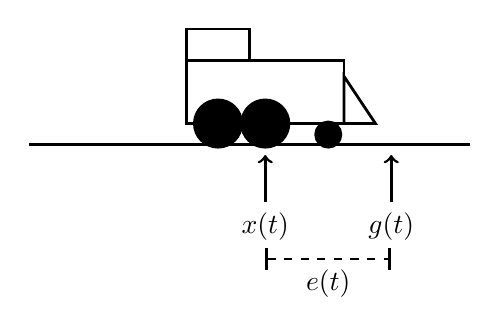
\begin{tikzpicture}
[line width=1pt,rotate=0,scale=.4]

\filldraw (2.0, 1) circle (.75);
\filldraw (3.5, 1.0) circle (.75);
\filldraw (5.5, .65) circle (.4);

\draw (1,1) -- (6,1) -- (6,3) -- (1, 3) -- cycle; %body
\draw (1,3) -- (3,3) -- (3,4) -- (1, 4) -- cycle; %cab
\draw (6,1) -- (7,1) -- (6,2.5)  -- cycle; %plow
\draw (-4, .325) -- (10, .325); %rails

\draw[->] (3.5, -1.5)  node [anchor=north]{$x(t)$} -- (3.5,0);
\draw[->] (7.5, -1.5)  node [anchor=north]{$g(t)$} -- (7.5,0);

\draw[|-|] (3.5, -3.3)[dashed] -- (7.5,-3.3) node[pos=0.5,below]{$e(t)$};



\end{tikzpicture}
\end{center}
\caption{A self-driving locomotive.}
\label{fig:locomotive2}
\end{figure}


The problems with the naive controller in Algorithm
\ref{lst:open-loop} can be avoided by using \vocab{closed loop
  control}\index{closed loop control}.  Closed loop controllers
continuously monitor the current error in the system and update the
control signal to push the error toward zero.  This approach tends to
be more reliable because the controller responds to the actual state
of the system and is able to make adjustments when the system fails to
behave as expected.


The PID (\textbf{P}roportional, \textbf{I}nverse, \textbf{D}erivative)
controller is the classic example of closed loop control.  The next
several sections will introduce the PID controller by describing each
of these three terms.  The following table outlines the notation
that will be used (Figure
\ref{fig:locomotive2} also uses this notation).


\begin{tabular}{l p{4in}}
$x(t)$ &

  The state of the system at time $t$.  In the case of the locomotive
  this is the position on the track. More generally, this could
  describe any state variable that we are interested in controlling.
  This could be the temperature of a room or the altitude of a
  rocket.

  For now, we will assume that state information is provided by a
  reliable sensor.  In future chapters we will consider the problem of
  estimating this value when sensors are absent or unreliable.\\

$g(t)$ & Goal state at time $t$. \\

$e(t)$ & Error at time $t$.

 We will let $e(t) = g(t) - x(t)$. In the case of the locomotive, this
 value is zero when the locomotive is at the goal position, positive
 when the locomotive is to the left of the goal, and negative if the
 locomotive overshoots and ends up to the right of the goal. \\

$u(t)$ & The control signal at time $t$. The interpretation of $u(t)$
 depends on system we are attempting to control.  In some cases $u(t)$
 might represent a low-level control signal like the voltage sent to a
 motor. In other cases we may be working with a robot that allows us
 to directly specify a desired velocity or acceleration.

 In the case of our hypothetical locomotive, we will assume we have an
 API provides a \verb+throttle+ function that takes a number in the
 range (-100, 100) where +100 represents ``full speed ahead'' and -100
 represents ``full reverse''.
\end{tabular}

\subsection{Proportional Control}

Mathematically, we can think of the problem of developing a controller
as finding an expression for $u(t)$ in terms of $e(t)$.  One simple
possibility is to follow the intuition that the magnitude of the control
signal should be proportional to the current error.  In the locomotive
example, this means we should apply more throttle when the locomotive
is far from the goal location, and ease off as the locomotive gets
closer.  This idea can be expressed as follows:

\begin{equation}
 u(t) = K_p e(t)
\end{equation}

The value $K_p$ is referred to as a \vocab{gain}\index{gain} term. This is a
constant that determines how large the control signal will be for a
particular error value.  Doubling the gain doubles the magnitude of
the control signal.  Developing a successful controller involves
selecting an appropriate gain value, either by analyzing the system or
through trial and error.

Algorithm \ref{lst:proportional} shows how we can implement a
proportional controller for the locomotive example.


\begin{minipage}[c]{0.95\textwidth}
\begin{lstlisting}[label={lst:proportional},caption={Proportional Control Algorithm}]
def p_controller(train, g, K_P):
    while True:
        e = g - train.x
        u = K_P * e
        train.throttle(u)

\end{lstlisting}
\end{minipage}



Figure \ref{fig:p_result} shows the result of using a proportional
controller to implement our locomotive controller using two different
values of $K_P$.

\begin{figure}
\includegraphics{pid/figs/p_result.pdf}
\caption{Locomotive position error over time for two different values of $K_P$.} 
\label{fig:p_result}
\end{figure}

These results are not very satisfying. The locomotive overshoots the
goal and then over-corrects, driving back and forth indefinitely.
Changing the value of $K_P$ doesn't solve the problem, it only changes
the period of the oscillations.


\subsection{Adding a Derivative Term}

One problem with our proportional controller is that it only considers
the position of the locomotive, not the speed.  Intuitively, it seems
that if the error is already decreasing quickly, we should reduce the
control signal to avoid overshooting the goal.  Conversely, if the
error is still increasing in spite of the proportional control, we should
further increase the magnitude of the control signal.  These
intuitions can be captured by adding a derivative term to the
controller:

\begin{equation}
u(t) = K_p e(t) +
\tikz[baseline]{
    \node[draw=red,rounded corners,anchor=base] (m1)
    {$\displaystyle K_d \diff{e(t)}{t}$};
    \node[above of=m1] (l1) {derivative term};
    \draw[-,red] (l1) -- (m1);
}
\label{eq:pd_equation}
\end{equation}


The term $\diff{e(t)}{t}$ describes the rate of change in the error.
This is negative if the error is decreasing and positive if the error
is increasing.  The value $K_d$ is a gain that is used to tune
the impact of the derivative term.

Using the derivative term requires us to know $\diff{e(t)}{t}$, but
sensors don't usually provide direct access to this value.  Instead,
we need to estimate it by tracking the change in error over time.
Even though the physical systems we are controlling operate
continuously, our algorithms necessarily perform their steps at
discrete time intervals.  Assuming our controller is updated every
$\Delta t$ seconds, we can estimate the derivative as the slope
between the two most recent error values:

\begin{equation}
\diff{e(t)}{t} \approx \frac{e(t) - e(t - \Delta t)}{\Delta t}
\label{eq:diff_approx}
\end{equation}


% Issue: approximation can cause problems if delta t is short and 
% measurements are noisy.

%% \begin{tikzpicture} 
%% \begin{axis}[ 
%% height=5cm, 
%% width=5cm, 
%% xlabel=$t$, 
%% ylabel=$e(t)$,
%% xmin=0, 
%% xmax=2, 
%% samples=10,
%% smooth,] 

%% \addplot [domain=0:2,mark=]{10 *x^3 + 1 - 3* x^2}; 

%% \end{axis} 
%% \end{tikzpicture}


Discrete approximations like this are common in robotics and in
other areas of scientific computing but they aren't always made
explicit.  It takes some experience to get comfortable moving from
continuous to discrete formulations. Algorithm
\ref{lst:proportional_deriv} illustrates how we can use the discrete
approximation in Equation \ref{eq:diff_approx} to implement the
control algorithm described in Equation \ref{eq:pd_equation}. 


\begin{minipage}[c]{0.95\textwidth}
\begin{lstlisting}[label={lst:proportional_deriv},caption={Proportional Derivative Control Algorithm}]
def pd_controller(train, g, K_P, K_D):
    e_prev = g - train.x
    while True:
        e = g - train.x
        dedt = (e - e_prev) / train.dt  # Equation 1.3
        u = K_P * e + K_D * dedt
        train.throttle(u)
        e_prev = e
\end{lstlisting}
\end{minipage}


\begin{figure}
\includegraphics{pid/figs/pd_result.pdf}
\caption{Locomotive position error over time for three different
  values of $K_D$.}
\label{fig:pd_result}
\end{figure}

Figure \ref{fig:pd_result} shows the result of introducing the derivative term in our
controller.  For appropriate values of $K_D$ the oscillations are
damped, and the locomotive settles at the goal location.

\subsection*{Stop and Think}

\begin{exercise}
  The \verb+while+ loop in Listing \ref{lst:proportional_deriv} does
  not include any explicit delays.  It is written under the assumption
  that methods called on the \verb+train+ object will only return
  after an appropriate delay.  What could go wrong if this is not the
  case?  In other words, what will happen if the execution time of the
  loop is much shorter than \verb+train.dt+?
\end{exercise}



\subsubsection{Droop}


\begin{figure}
\begin{center}
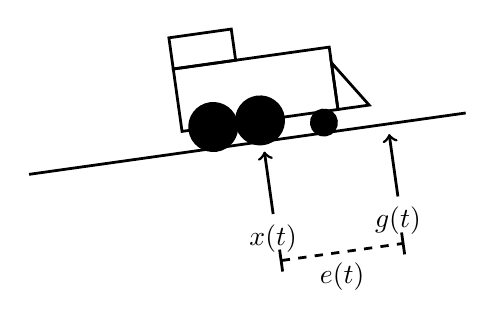
\begin{tikzpicture}
[line width=1pt,rotate=8,scale=.4]

\filldraw (2.0, 1) circle (.75);
\filldraw (3.5, 1.0) circle (.75);
\filldraw (5.5, .65) circle (.4);

\draw (1,1) -- (6,1) -- (6,3) -- (1, 3) -- cycle; %body
\draw (1,3) -- (3,3) -- (3,4) -- (1, 4) -- cycle; %cab
\draw (6,1) -- (7,1) -- (6,2.5)  -- cycle; %plow
\draw (-4, .325) -- (10, .325); %rails

\draw[->] (3.5, -2)  node [anchor=north]{$x(t)$} -- (3.5,0);
\draw[->] (7.5, -2)  node [anchor=north]{$g(t)$} -- (7.5,0);

\draw[|-|] (3.5, -3.5)[dashed] -- (7.5,-3.5) node[pos=0.5,below]{$e(t)$};
\end{tikzpicture}
\end{center}
\caption{Locomotive on a hill.}
\label{fig:train_hill}
\end{figure}

What happens when we try to apply the same controller when the
locomotive is located on a slight incline as shown in Figure
\ref{fig:train_hill}?  In this situation, which is illustrated in
Figure \ref{fig:pd_droop}, the locomotive never quite
reaches the goal position.  The locomotive comes to rest at the point
where the proportional force applied by the controller is exactly
counterbalanced by gravity.  Increasing $K_p$ will move the stationary
point closer to the goal, but this controller will never drive the
error all the way to zero.  The situation where the proportional term
is not sufficient to drive the error term to zero is sometimes
referred to as ``droop''. 

\begin{figure}
\includegraphics{pid/figs/pd_result_hill.pdf}
\caption{Locomotive position error over time for the PD locomotive
  controller when the locomotive is on an incline.  The locomotive
  stops short of the goal at the point where the control output is
  counter-balanced by gravity.}
\label{fig:pd_droop}
\end{figure}



\subsection{Adding an Integral Term}

The problem of droop can be addressed by adding one more term to our
controller:

\begin{equation}
u(t) = K_P e(t) +
\tikz[baseline]{
    \node[draw=red,rounded corners,anchor=base] (m1)
    {$\displaystyle K_I  \int_0^t e(\tau)d\tau $};
    \node[above of=m1] (l1) {integral term};
    \draw[-,red] (l1) -- (m1);
}
+ K_D \diff{e(t)}{t} 
\end{equation}

\noindent Where the derivative term allows the controller to look forward in
time, the integral term allows the controller to look backwards in
time.  The integral $\int_0^t e(\tau)d\tau$ essentially ``stores up''
the error that the system sees over time.  As long as the error fails
to reach zero, $\int_0^t e(\tau)d\tau$ will steadily increase in
magnitude.

As with the derivative, the integral value is not available directly,
but must be estimated from discrete samples.  In this case, the
integral can be estimated using a summation that adds the current
error value at each time step:


\begin{equation}
\includegraphics{pid/figs/annotated_summation.pdf}
%\int_0^t e(\tau)d\tau \approx \sum_{i=0}^{t/\Delta t} e(i \Delta t) \Delta t 
\end{equation}

%% \begin{tikzpicture}
%% \begin{axis}[
%%  ylabel near ticks,
%%     xtick={0,1,3,5,7,9,11,13,15,17},ytick={0,...,1.5},
%%     xmax=18,ymax=1.2,ymin=0,xmin=0,
%%     enlargelimits=true,
%%     axis lines=middle,
%%     clip=false,
%%     domain=0:17,
%%     xlabel near ticks,
%%     xlabel={$t$},
%%     ylabel={$e(t)$},
%%     ]

%% \addplot [draw=red, fill=red!10, ybar interval, samples=9, domain=1:17]
%%     {x^-1}\closedcycle;

%% \addplot[smooth, thick,domain=1:17,samples=40]{x^-1};

%% \end{axis}
%% \end{tikzpicture}




\begin{minipage}[c]{0.95\textwidth}
\begin{lstlisting}[label={lst:pid},caption={PID Control Algorithm}]
def pid_controller(train, g, K_P, K_I, K_D):

    e_prev = g - train.x
    e_sum = 0             # accumulator for integral term
    while True:
        e = g - train.x
        e_sum = e_sum + e * train.dt   # From Equation 1.5
        dedt = (e - e_prev) / train.dt # Equation 1.3 
        u = K_P * e   +   K_I * e_sum   +   K_D * dedt
        train.throttle(u)
        e_prev = e

\end{lstlisting}
\end{minipage}


\begin{figure}
\includegraphics{pid/figs/pid_result_hill.pdf}
\caption{Locomotive position error over time for a different slopes.
  With appropriate gain values the PID controller reliably moves the
  locomotive to the goal location.}
\label{fig:pid_result}
\end{figure}


Algorithm \ref{lst:pid} illustrates a complete PID controller.  Figure
\ref{fig:pid_result} shows the result of adding an integral term to
our locomotive controller.  With an appropriate value of $K_I$, the
resulting controller reliably moves the locomotive to the goal regardless
of the slope.

\subsection*{Stop and Think}
\begin{exercise}
  Practical implementations of PID controllers often place a cap on
  the amount of error that can be accumulated in the integral term of
  the controller.  Why do you think this is necessary?  What could go
  wrong if the controller were to start out far from the goal
  configuration, accumulating a large amount of error before the goal
  is reached?
\end{exercise}

\begin{exercise}
  The process outlined above for tuning the PID gain terms is ad-hoc:
  we just experimented with different values until the behavior looked
  right. A more rigorous approach would require a quantitative way to
  evaluate the success of a particular PID controller.  Can you think
  of some quantitative measurements that might be useful for comparing
  two controllers? 
\end{exercise}


\begin{exercise}
  Consider the following graph of error as a function of
  time. Assuming that this system is being controlled by a PID
  controller, how would you suggest what the gain terms be modified?
  \begin{center}
  \includegraphics[width=2.2in]{pid/figs/pid_stop_and_think1.pdf}
  \end{center}
\end{exercise}

\begin{exercise}
  Consider the following graph of error as a function of
  time. Assuming that this system is being controlled by a PID
  controller, how would you suggest what the gain terms be modified?
  \begin{center}
  \includegraphics[width=2.2in]{pid/figs/pid_stop_and_think2.pdf}
  \end{center}
\end{exercise}


%% \subsection{complictions}
%% Calculating derivative
%% Storing derivatives
%% Tuning gains

%% restricting the magnitude

\section{Proportional Robot Control}
\label{sec:p_robot_control}
%---------------------------------
% MACROS FOR DRAWING ROBOTS
%--------------------------------
\newcommand{\drawwheel}[2]{
\begin{scope}[shift={(#1,#2)}]
\filldraw (.3,.1) -- (.3,-.1) -- (-.3,-.1) -- (-.3,.1) -- cycle; 
\end{scope}
}

%Draw robot at x, y, theta
\newcommand{\drawdiffrobot}[4]{
\begin{scope}[shift={(#1,#2)},rotate=#3,scale=#4]
\draw (0,0) circle (1);
\draw[thick,->] (0,0) -- (.7,0);
\drawwheel{0}{.7}
\drawwheel{0}{-.7}
\end{scope}
}

%---------------------------------
%--------------------------------



You may feel that a self-driving locomotive is a disappointingly
simple robot: all it can do is move backward and forward along a
linear track.  Don't fear, this book will mostly focus on mobile
robots that are able to move freely in multiple dimensions.  In this
section we will develop a proportional controller for driving a wheeled
robot to a goal location as illustrated in Figure
\ref{fig:diff_robot}.



\begin{figure}[h]
\begin{center}
\includegraphics{pid/figs/3drobot.png}
\end{center}
\caption{Differential drive robot.}
\label{fig:diff_robot}
\end{figure}



%% \begin{figure}[h]
%% \begin{center}
%% \begin{tikzpicture}

%% \coordinate[] (G) at (3.5,1);
%% \coordinate[] (R) at (1, 2);

%% %Axes
%% \draw[thick,->] (0,0) -- (4.5,0) node[anchor=north ] {$x$};
%% \draw[thick,->] (0,0) -- (0,4.5) node[anchor= east] {$y$};

%% %Robot
%% \drawdiffrobot{1}{2}{45}{.4}

%% %Robot label
%% \draw[->,shorten >=0.6cm] (1.78,3.08) node[above] {Robot} -- (R);

%% %Star
%% \draw (G) node[draw,star,star points=5,star point ratio=.5]{};

%% %Star label
%% \draw[->,shorten >=0.4cm] (4.5, 2) node[above] {Goal} -- (G);

%% \end{tikzpicture}
%% \end{center}
%% \caption{Overhead view of a differential drive robot.  The small black
%%   rectangles represent the wheels.}
%% \label{fig:diff_robot}
%% \end{figure}


This is an example of a \vocab{differential drive}\index{differential
  drive} robot.  This type of robot has two independently controllable
wheels.  When both wheels are rotated in the same direction at the
same speed the robot moves directly forward or backward.  If both
wheels are turned in opposite directions the robot will rotate in
place.  The robot can follow a curved path by rotating each wheel at a
different speed.

Since it is not intuitive to steer a differential drive robot by
directly controlling the wheel velocities, the driver software for
such robots often accepts commands specifying two velocity values: $v$
and $w$, where $v$ is the forward velocity in meters/second and $w$ is
the rotational velocity in radians/second. 
%TODO call forward to kinematics chapter where this translation will
%be described.

\begin{figure}[h!]
\begin{center}
\begin{tikzpicture}

\node[] (G) at (3.5,1){};
\coordinate[] (R) at (1, 2);
\coordinate[] (xaxis) at (4.5,0);
\coordinate[] (yaxis) at (0, 4.5);

% Axes
\draw [<->,thick] (yaxis)node[label=left:$y$] {} |- 
(xaxis)node[label=below:$x$] {};

% Robot
\drawdiffrobot{1}{2}{45}{.4}

\begin{scope}[draw=blue,text=blue]
% x, y coordinates
\draw[dashed,shorten >=0.4cm] (yaxis |- R) node[left] {$y_r$} -- (R);
\draw[dashed,shorten >=0.4cm] (xaxis -| R) node[below] {$x_r$} -- (R);

% angle:
\coordinate[] (A) at ($(R) + (1.75,1.75)$);
\coordinate[] (C) at ($(R) + (2,0)$);
\draw[dashed,->,shorten <=0.4cm] (R) node[above] {} -- (A);
\draw[dashed,->,shorten <=0.4cm] (R) node[above] {} -- (C);
\tkzMarkAngle[arc=l,size=1.0,arrows=->](C,R,A)
\tkzLabelAngle[pos = 1.3](C,R,A){$\Theta_r$}
\end{scope}

%Star
\draw (G) node[draw,star,star points=5,star point ratio=.5]{};

\begin{scope}[draw=green,text=green]
% x, y coordinates
\draw[dashed] (yaxis |- G) node[left] {$y_g$} -- (G);
\draw[dashed] (xaxis -| G) node[below] {$x_g$} -- (G);
\end{scope}


\end{tikzpicture}
\end{center}
\caption{Overhead view of the robot and goal.}
\label{fig:diff_coords}
\end{figure}

Figure \ref{fig:diff_coords} illustrates the parameterization of the
control problem.  The pose of the robot is specified with three
numbers: $(x_r, y_r, \Theta_r)$, where the $x_r$ and $y_r$ coordinates
specify the position of the center of the robot with respect to some
fixed point in the room and the $\Theta_r$ value indicates the robot's
heading.  Heading values (in radians) are in the interval $[-\pi,
  \pi]$, where $\Theta_r = 0$ indicates that the robot is pointing
along (or parallel to) the $x$-axis.
As the robot turns counterclockwise, $\Theta_r$ increases.
The value of $\Theta_r$ in figure
Figure \ref{fig:diff_coords} is approximately $\frac{\pi}{4}$ (or
$45^o$).



We can solve this control problem by creating two separate
proportional controllers that will operate simultaneously: one
controller to output a rotational velocity that turns the robot toward
the goal, the other to output a forward velocity that keeps the robot
moving forward until it reaches the goal.


\begin{figure}[h!]
\begin{center}
\begin{tikzpicture}

\node[] (G) at (3.5,1){};
\coordinate[] (R) at (1, 2);
\coordinate[] (xaxis) at (4.5,0);
\coordinate[] (yaxis) at (0, 4.5);

% Axes
\draw [<->,thick] (yaxis)node[label=left:$y$] {} |- 
(xaxis)node[label=below:$x$] {};

% Robot
\drawdiffrobot{1}{2}{45}{.4}

% Star
\draw (G) node[draw,star,star points=5,star point ratio=.5]{};

% Triangle
\coordinate[] (A) at (R -| G);
\draw (A) -- node[above] {$x_g - x_r$} (R) -- (G) -- 
node[right] {$y_g - y_r$}(A);

% Label angle.
\tkzMarkAngle[arc=l,size=1.0,arrows=<-](G,R,A)
\tkzLabelAngle[pos = 1.3](G,R,A){$\Theta_g$}
\end{tikzpicture}

\end{center}
\caption{Goal angle calculations}
\label{fig:goal_angle}
\end{figure}

The first step in developing the rotational controller is determining
the desired angle for the robot.  The problem is illustrated in Figure
\ref{fig:goal_angle}. Determining $\Theta_g$ from the positions of the
robot and goal requires some trigonometry:

\begin{equation}
\Theta_g = \tan^{-1}  \frac{y_g - y_r}{x_g - x_r}
\label{eq:calc_theta_g}
\end{equation} 

Actually, this won't \emph{quite} give us what we want.  Equation
\ref{eq:calc_theta_g} doesn't distinguish between the case when both
the numerator and denominator are positive and the case when they are
both negative.  This means that a goal above and to the right of the
robot will result in the same angle as an object below and to the
left.  The math libraries for many programming languages address this
difficulty by providing a function named \texttt{atan2} that takes the
numerator and denominator as separate arguments and correctly
calculates the angle taking the signs of the arguments into account.
A Python implementation might look something like the following:

\begin{center}
\begin{verbatim}
theta_g = math.atan2(y_g - y_r, x_g - x_r)
\end{verbatim}
\end{center}

Given that we can calculate a target angle, our rotational controller
can be specified using the formula for a proportional controller
(dropping the time index for clarity):


\begin{equation}
 w = K_{P_w} (\Theta_g - \Theta_r)
\end{equation}

Unfortunately, subtracting angles in a sensible way requires some
caution.  Consider the situation in Figure \ref{fig:angle_problem}.
Naively calculating the error by subtracting the two angles gives us
$.9 \pi - (-.9\pi) = 1.8\pi$.  Plugging this into our proportional
controller will result in a hard left turn.  This isn't exactly wrong:
it \emph{is} possible for the robot to point toward the goal by
turning to the left.  However, it clearly makes more sense to select
the smaller angle between our current heading and the target heading and
have the robot turn right.
We will use the symbol $\ominus$ to indicate an angle subtraction
operation that has this effect.  With this modification we can
completely specify the control scheme for the differential drive
robot.

\begin{align} 
 w =& K_{P_w} (\Theta_g \ominus \Theta_r) \label{eq:diff_rot}\\
 v =& K_{P_v} \sqrt{(y_g - y_r)^2 + (x_g - x_r)^2} \label{eq:diff_vel}
\end{align}

Equation \ref{eq:diff_vel} expresses the idea that the robot's forward
velocity should be proportional to its Euclidean distance from the
goal.  Since this velocity control is independent of the angle, the
robot may initially move away from the goal.  We could address through
a more complicated control mechanism, but the point here is to
illustrate a simple example of proportional control.  Figure
\ref{fig:diff_demo} shows several example trajectories of a simulated
differential drive robot under the control scheme presented in
Equations \ref{eq:diff_rot} and \ref{eq:diff_vel}.


\begin{figure}[h!]
\begin{center}
\begin{tikzpicture}

\node[] (G) at (1,2.81){};
\coordinate[] (R) at (3.5, 2);
\coordinate[] (xaxis) at (4.5,0);
\coordinate[] (yaxis) at (0, 4.5);

% Axes
\draw [<->,thick] (yaxis)node[label=left:$y$] {} |- 
(xaxis)node[label=below:$x$] {};

% Robot
\drawdiffrobot{3.5}{2}{-162}{.4}

% Star
\draw (G) node[draw,star,star points=5,star point ratio=.5]{};

% angle:
\coordinate[] (C) at ($(R) + (2,0)$);
\draw[dashed,->,shorten <=0.4cm] (R) node[above] {} -- (C);

% goal angle
\begin{scope}[draw=green,text=green]
\draw[dashed,->,shorten <=0.4cm] (R) node[above] {} -- (G);
\tkzMarkAngle[arc=l,size=1.0,arrows=->](C,R,G)
\tkzLabelAngle[pos = 1.3](G,R,C){$\Theta_g = .9\pi$}
\end{scope}

% robot angle
\coordinate[] (D) at ($(R) + (-2,-.65)$);
\begin{scope}[draw=blue,text=blue]
\draw[dashed,->,shorten <=0.4cm] (R) node[above] {} -- (D);
\tkzMarkAngle[arc=l,size=.8,arrows=<-](D,R,C)
\tkzLabelAngle[pos = 1.3](D,R,C){$\Theta_r = -.9\pi$}
\end{scope}

\end{tikzpicture}

\end{center}
\caption{The robot can either turn $.2\pi$ radians clockwise, or $1.8\pi$ radians
  counterclockwise to face the goal. We want a difference operation
  that always returns the smaller angle. }
\label{fig:angle_problem}
\end{figure}


\begin{figure}[h!]
\begin{center}
\begin{tikzpicture}
\begin{axis}[unit vector ratio*=1 1 1,
axis x line=bottom,
axis y line=left,
xmin=1.5,xmax=9,
ymin=1.5,ymax=9.25,
ticks=none]
\addplot[color=red,smooth] coordinates {
(7.43698072433, 3.02302646637)
(7.30944538116, 2.8852930069 )
(7.12435770035, 2.84149670601)
(6.90518760681, 2.88129091263)
(6.73256778717, 2.96469521523)
(6.57478523254, 3.07387018204)
(6.42918539047, 3.19893813133)
(6.27081918716, 3.35729455948)
(6.14221286774, 3.49984359741)
(6.01804590225, 3.6462829113)
(5.87715482712, 3.82042050362)
(5.75883102417, 3.97162556648)
(5.64206647873, 4.12403869629)
(5.52646827698, 4.27733898163)
(5.39273405075, 4.45703601837)
(5.27888917923, 4.61164283752)
(5.17062282562, 4.75992250443)
(5.10430622101, 4.85154008865)
(5.05697059631, 4.9176197052)
(5.03474617004, 4.949010849)
(5.02116727829, 4.96842718124)
 };


\addplot[color=red,smooth] coordinates {
(8.22, 5.54)
(8.13, 5.71)
(7.98, 5.81)
(7.79, 5.87)
(7.57, 5.88)
(7.38, 5.86)
(7.19, 5.82)
(7.01, 5.77)
(6.79, 5.70)
(6.61, 5.64)
(6.43, 5.58)
(6.25, 5.51)
(6.04, 5.43)
(5.86, 5.36)
(5.68, 5.28)
(5.48, 5.20)
(5.30, 5.13)
(5.18, 5.08)
(5.11, 5.05)
(5.06, 5.03)
(5.04, 5.02)
};

\addplot[color=red,smooth] coordinates {
(6.50, 8.72)
(6.70, 8.77)
(6.84, 8.65)
(6.91, 8.47)
(6.92, 8.28)
(6.88, 8.06)
(6.81, 7.88)
(6.73, 7.71)
(6.64, 7.54)
(6.53, 7.34)
(6.44, 7.18)
(6.33, 7.01)
(6.21, 6.82)
(6.11, 6.66)
(6.00, 6.50)
(5.90, 6.34)
(5.77, 6.16)
(5.67, 6.00)
(5.56, 5.84)
(5.45, 5.68)
(5.33, 5.49)
(5.22, 5.33)
(5.14, 5.20)
(5.08, 5.13)
(5.04, 5.06)
(5.03, 5.04)
};
\addplot[color=red,smooth] coordinates {
(3.34, 7.82)
(3.53, 7.80)
(3.70, 7.71)
(3.87, 7.56)
(3.98, 7.41)
(4.09, 7.25)
(4.18, 7.08)
(4.28, 6.88)
(4.35, 6.70)
(4.43, 6.53)
(4.51, 6.32)
(4.58, 6.14)
(4.65, 5.96)
(4.72, 5.78)
(4.79, 5.57)
(4.86, 5.39)
(4.91, 5.24)
(4.95, 5.15)
(4.97, 5.08)
(4.98, 5.05)
(4.99, 5.03)
};
\addplot[color=red,smooth] coordinates {
(2.49, 5.93)
(2.51, 5.74)
(2.61, 5.58)
(2.78, 5.43)
(2.95, 5.34)
(3.13, 5.27)
(3.31, 5.22)
(3.53, 5.17)
(3.72, 5.13)
(3.91, 5.10)
(4.10, 5.08)
(4.32, 5.05)
(4.51, 5.03)
(4.70, 5.02)
(4.83, 5.01)
(4.90, 5.00)
(4.94, 5.00)
(4.96, 5.00)
};
\addplot[color=red,smooth] coordinates {
(2.50, 3.17)
(2.69, 3.14)
(2.88, 3.16)
(3.09, 3.24)
(3.25, 3.33)
(3.41, 3.44)
(3.56, 3.56)
(3.73, 3.71)
(3.87, 3.84)
(4.01, 3.97)
(4.17, 4.13)
(4.30, 4.27)
(4.44, 4.41)
(4.57, 4.54)
(4.73, 4.71)
(4.83, 4.82)
(4.90, 4.89)
(4.94, 4.93)
(4.97, 4.96)
(4.98, 4.98)
};

\addplot[color=red,smooth] coordinates {
(5.21, 2.26)
(5.08, 2.13)
(4.89, 2.15)
(4.72, 2.29)
(4.64, 2.46)
(4.59, 2.64)
(4.57, 2.84)
(4.58, 3.06)
(4.60, 3.25)
(4.63, 3.44)
(4.66, 3.63)
(4.71, 3.85)
(4.75, 4.04)
(4.79, 4.22)
(4.85, 4.44)
(4.89, 4.63)
(4.93, 4.77)
(4.96, 4.86)
(4.98, 4.92)
(4.98, 4.95)
(4.99, 4.97)
};

\node[inner sep=0pt] (russell) at (axis cs:7.437,3.023)
    {\includegraphics[angle=251,scale=.6]{pid/robot.pdf}};

\node[inner sep=0pt] (russell) at (axis cs:8.22,5.54)
    {\includegraphics[angle=96,scale=.6]{pid/robot.pdf}};

\node[inner sep=0pt] (russell) at (axis cs:6.50,8.72)
    {\includegraphics[angle=57,scale=.6]{pid/robot.pdf}};

\node[inner sep=0pt] (russell) at (axis cs:3.34,7.82)
    {\includegraphics[angle=9,scale=.6]{pid/robot.pdf}};

\node[inner sep=0pt] (russell) at (axis cs:2.49,5.93)
    {\includegraphics[angle=258,scale=.6]{pid/robot.pdf}};

\node[inner sep=0pt] (russell) at (axis cs:2.50,3.17)
    {\includegraphics[angle=335,scale=.6]{pid/robot.pdf}};

\node[inner sep=0pt] (russell) at (axis cs:5.21,2.26)
    {\includegraphics[angle=265,scale=.6]{pid/robot.pdf}};

\draw (axis cs:5,5) node[fill=white,draw,star,star points=5,star point ratio=.5]{};

\end{axis}
\end{tikzpicture}
\end{center}
\caption{Example trajectories for a proportional controller that moves
  a differential drive robot to a goal location.  The robot images
  indicate the starting positions for seven simulated navigation
  trials.}
\label{fig:diff_demo}
\end{figure}


Notice that, unlike the locomotive example, it wasn't necessary to
include integral or derivative terms in this controller.  They
weren't needed because we were able to set the speed of the
robot directly. This means we didn't need to worry as much about
overshooting the goal or applying too little force to reach it.  It
often makes sense to start with a pure proportional controller and add
integral or derivative terms if they prove necessary.

\section{Limitations of PID Controllers}

PID control is widely used because it is simple to implement and can
be applied in a wide range of situations.  We can use PID control even
when we don't have an accurate model of the system we are controlling.
In this chapter we used trial and error to develop a PID controller
for a simulated locomotive.  It wasn't necessary to understand the
physics involved: we didn't need to estimate frictional forces, we
didn't need an exact specification of the forces created by the
throttle.  We only needed to tune the three gain parameters until we
were satisfied with the performance.

The ad-hoc nature of PID control can also be seen as a disadvantage.
PID controllers tend to work well in practice, but they don't provide
any optimality guarantees.  In cases where we \emph{do} have an
accurate system model, it's possible to develop more principled
controllers that explicitly minimize a cost function related to the
quality of the solution.  This could allow us to create a controller
that reaches the goal in the minimum time or with minimal energy
expenditure.  Such controllers are beyond the scope of this book, but
the classic optimal controller is the \vocab{Linear Quadratic
  Regulator} or LQR.

More significantly, the kind of low-level control discussed in this
chapter is obviously not appropriate for complex control problems that
extend over longer periods of time.  A PID controller will not save
the day for the robot in Figure \ref{fig:maze}.  Problems like this
will require planning algorithms of the sort described in Chapter \ref{chap:planning}.

\begin{figure}[h!]
\begin{center}
\begin{tikzpicture}



\node[inner sep=0pt] (R) at (-3,-.2)
    {\includegraphics[angle=0,scale=.6]{pid/robot.pdf}};

%\draw ($(R) + (-.8, .8)$) node[draw,ellipse] {???};
\draw ($(R) + (-.5, .4)$) node[draw,ellipse,inner sep=0pt,minimum size=.6em] {};
\draw ($(R) + (-.35, .25)$) node[draw,ellipse,inner sep=0pt,minimum size=.3em] {};
\draw ($(R) + (-.8, 1)$) node [cloud, draw,cloud puffs=10,cloud puff arc=120, aspect=4, inner ysep=0em, minimum size=3em] {???};

% Star
\draw (3,.2) node[draw,star,star points=5,star point ratio=.5]{};

\node[inner sep=0pt] (M) at (0,0)
    {\includegraphics[angle=90,scale=1.1]{pid/figs/maze.pdf}};

\end{tikzpicture}

\end{center}
\caption{A control problem that can't be solved with the tools in this chapter.}
\label{fig:maze}
\end{figure}

\section{References and Further Reading}

\subsection{Closed-Loop Controllers}

Elements of the PID control model have been in place since the time of
the industrial revolution.  A history of the development of PID
control theory since 1900 is provided in \parencite{BENNETT200143}.
PID controllers are widely used in both robotics and industrial
automation, and as such, there is a huge literature on tuning and
implementing PID controllers. A recent 500-page reference can be found
in \parencite{johnson2006pid}.

A standard reference on the Linear Quadratic Regulator is
\parencite{anderson2007optimal}.

\subsection{General Robotics Resources}

There are a huge number of robotics textbooks and references.  I will
highlight a few here that are particularly notable and were useful in
the development of this book.

The most widely used artificial intelligence textbook is
\parencite{Russell2003}. While that book has a broader scope than just
robotics, many areas of AI are directly relevant to robotics
work. Another excellent general AI textbook is
\parencite{PooleMackworth17}.  This book has the advantage of being
available online at no cost: \url{https://artint.info/}.

\emph{Computational Principles of Mobile Robotics}
\parencite{dudek2010} is a robotics textbook that has a similar focus
to this work: it is targeted to computer scienists and focuses on
algorithmic issues in robotics.  An excellent open-access robotics
textbook is \parencite{correll2022introduction}.  The definitive work
on probalistic methods in robotics is \emph{Probalistic Robotics}
\parencite{thrun2005}.  An excellent, and authoritative, reference on
many topics in robotics is provided by the \emph{Springer Handbook of
  Robotics} \parencite{siciliano2008}.

%\section{Exercises}
